\subsection{Dill}
\label{sec:dill}

\begin{spice}\label{spice:dill}
\textsc{Dill} \hfill \href{https://powo.science.kew.org/taxon/837530-1}{POWO} \\
\textbf{English:} \textit{dill}. 
\textbf{Arabic:} {\arabicfont{شبت}} \textit{shibitt}. 
\textbf{Chinese:} {\tradchinesefont{蒔蘿}} \textit{shíluó}. 
\textbf{Hungarian:} \textit{kapor}.  \\
\noindent{\color{black}\rule[0.5ex]{\linewidth}{.5pt}}
\begin{tabular}{@{}p{0.25\linewidth}@{}p{0.75\linewidth}@{}}
Plant species: & \taxonn{Anethum graveolens}{L.} \\
Family: & \textit{Apiaceae} \\
Plant part used: & fruit; leaf \\
Region of origin: & Nort Africa; West Asia \\
Cultivated in: & India \\
Color: & greyish brown \\
\end{tabular}
\end{spice}

\begin{figure}[!ht]
	\vspace{-4ex}
	\centering
	\subfloat[\centering a]{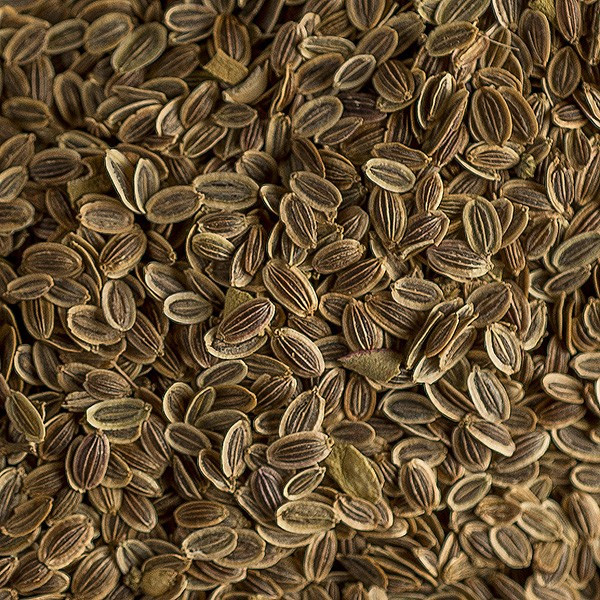
\includegraphics[width=0.3\linewidth]{imgs/spices/dill-1.jpg}}
	\hfill
	\subfloat[\centering b]{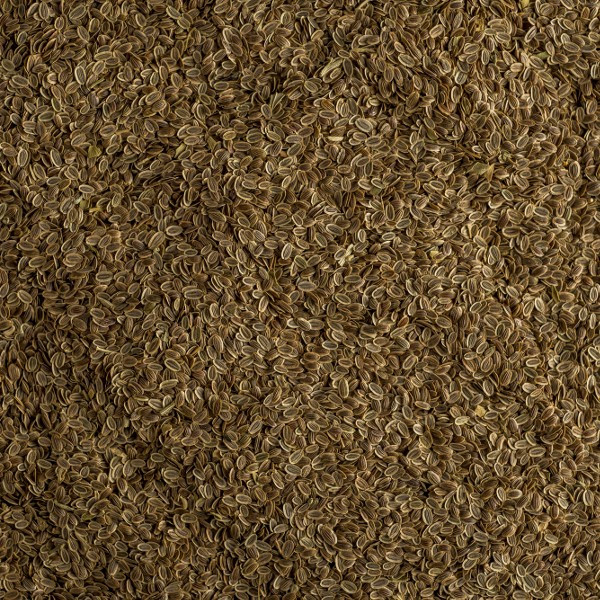
\includegraphics[width=0.3\linewidth]{imgs/spices/dill-2.jpg}}
	% \hfill
	% \subfloat[\centering c]{\includegraphics[width=0.3\linewidth]{imgs/spices/dill-3.jpg}}
	\caption{Dill \taxon{}.}
	\label{fig:dill_imgs}
\end{figure}

\subsection{The Botany of Dill}

\subsection{The History of Dill}

\subsection{The Names of Dill}

\subsubsection{English}

\begin{etymology}\label{ety:dill}
\textbf{English} \textit{dill}, ulterior derivation unknown, a. 700; cf. cognates  Old Low German \textit{dilli}, Dutch \textit{dille}, Old High German \textit{tilli}, Middle High German \textit{tille}, German \textit{dill, dille}, Danish \textit{dild}, Swedish \textit{dill} \footnote{\textcite[s.v. dill]{oed}}
\end{etymology}

\begin{table}[!ht]
    \caption{Various names for dill in English.}
\centering
\begin{tabularx}{\textwidth}{@{}l>{\itshape \small}lL>{\small}l@{}}
\toprule
\textbf{\#} & \multicolumn{1}{l}{\textbf{Species}} & \multicolumn{1}{l}{\textbf{Name}} & \multicolumn{1}{l}{\textbf{Source}} \\
\midrule
\textbf{1}	& \textbf{Anethum graveolens}	& \textbf{dill}	& \textbf{\textcite{van_wyk_culinary_2014}} \\
2	& Anethum graveolens	& dill-seed	& \textcite{oed} \\
3	& Anethum graveolens	& Indian dill	& \textcite{van_wyk_culinary_2014} \\
\bottomrule
\end{tabularx}
\label{table:names_dill_en}
\end{table}



\subsubsection{Arabic}

\begin{table}[!ht]
\centering
\begin{tabularx}{\textwidth}{@{}l>{\itshape \small}lr>{\itshape}lL>{\small}l@{}}
\toprule
\textbf{\#} & \multicolumn{1}{l}{\textbf{Species}} & \multicolumn{1}{l}{\textbf{Name}} & \multicolumn{1}{l}{\textbf{Tr.}} & \multicolumn{1}{l}{\textbf{Gloss}} & \multicolumn{1}{l}{\textbf{Source}} \\
\midrule
\textbf{1}	& \textbf{Anethum graveolens}	& \textbf{شبث}	& \textbf{shibithth}	& \textbf{}	& \textbf{\textcite{lane_arabic-english_1863}} \\
\bottomrule
\end{tabularx}
\caption{Various names for dill in Arabic.}
\label{table:names_dill_ar}
\end{table}



\subsubsection{Chinese}

\begin{table}[!ht]
\centering
\begin{tabularx}{\textwidth}{@{}l>{\itshape \small}ll>{\itshape}lL>{\small}l@{}}
\toprule
\textbf{\#} & \multicolumn{1}{l}{\textbf{Species}} & \multicolumn{1}{l}{\textbf{Name}} & \multicolumn{1}{l}{\textbf{Tr.}} & \multicolumn{1}{l}{\textbf{Gloss}} & \multicolumn{1}{l}{\textbf{Source}} \\
\midrule
\textbf{1}	& \textbf{Anethum graveolens}	& \textbf{\tradchinesefont{蒔蘿}}	& \textbf{shíluó}	& \textbf{phonetic}	& \textbf{} \\
2	& Anethum graveolens?	& \tradchinesefont{土茴香}	& tǔhuíxiāng	& earth-fennel	&  \\
\bottomrule
\end{tabularx}
\caption{Various names for dill in Chinese.}
\label{table:names_dill_zh}
\end{table}



\subsubsection{Summary}

\begin{table}[!ht]
\centering
\begin{tabularx}{\textwidth}{@{}ll>{\itshape}lLl>{\small}l@{}}
\toprule
\textbf{\#} & \textbf{Language} & \multicolumn{1}{l}{\textbf{Term}} & \textbf{Gloss} & \textbf{Loan} & \multicolumn{1}{l}{\textbf{Source}} \\
\midrule
1	& English	& dill	& 	& yes	& \textcite{oed} \\
2	& English	& dill-seed	& 	& no	& \textcite{oed} \\
\midrule
1	& Arabic	& shibithth	& 	& yes	& \textcite{lane_arabic-english_1863} \\
\midrule
\bottomrule
\end{tabularx}
\caption{Conventionalized names for dill in English, Arabic, and Chinese, found in dictionaries.}
\label{table:names_dill}
\end{table}
























% The word dill and its close relatives are found in most of the Germanic languages; its ultimate origin is unknown.[3] The generic name Anethum is the Latin form of Greek ἄνῑσον / ἄνησον / ἄνηθον / ἄνητον, which meant both 'dill' and 'anise'. The form anīsum came to be used for anise, and anēthum for dill. The Latin word is the origin of dill's names in the Western Romance languages (anet, aneldo, etc.), and also of the obsolete English anet.[4] Most Slavic language names come from Proto-Slavic *koprъ,[5] which developed from the PIE root *ku̯ə1po- 'aroma, odor'.[6]
